

\chapter{Methodology} \label{ch:methodology}
In this chapter ........

\section{Dataset}
A \gls{ds} could be defined as a structured collection of data that could be used for analysis, modeling and decision making. \gls{ds} exist in various formats, including numerical values, text, images and videos. In the scope of \gls{dl} and \gls{od}, a \gls{ds} is essential for training, validating and testing models. Moreover, the performance of an \gls{od} model highly depends on the quality and volume of the data available. Therefore, \gls{ds} collection and preparation is normally considered as the backbone of a high performance \gls{od} model. In \gls{od}, \gls{ds} primarily consist of images or video frames annotated with bounding boxes and labeled by classes to define the locations and categories of objects. For general \gls{od} tasks, one can use existing \gls{ds}s such as COCO, PASCAL VOC, and ImageNet which contain thousands of standardized and annotated images and video frames across multiple classes which are released over the last years. On the other hand, for solving highly specific tasks, a custom \gls{ds} may be required to train the model, making this step very complicated and time consuming step. However, using transfer learning and pre-trained models have reduced the need to collect thousands of images, as training with just a few hundred samples can result in a very satisfactory performance \cite{IBM_Transfer_Learning}. Additionally, modern annotation \gls{sw} available and different augmentation techniques help automate the process and scale up the \gls{ds} volume to deliver the best results. In this section, \gls{ds} collection, annotation and preprocessing techniques are discussed to collect high quality and volume \gls{ds} \cite{oD_Review}.

\subsection{Data Collection}
As stated earlier, \gls{od} algorithms heavily depend on the quality and volume of the data provided. This makes the \gls{dc} process a very important factor for the performance of the model. To reach good results, \gls{dc} process should follow a systematic approach consisting of multiple steps.

\subsubsection{Understanding Data Requirements}
The \gls{dc} process depends highly on the type of task to be performed. These tasks could be image segmentation, image classification, \gls{od}, facial recognition and pattern detection. Each one of these tasks require different type of \gls{ds} and understanding the task and clearly define the objectives are the fist steps in building the \gls{ds} \cite{AIMultiple_Computer_Vision_Training_Data}. In this study, as mentioned earlier, the focus is on \gls{od}, which involves image classification and localization.

Once the task is defined, the next step is to determine the appropriate training images and object categories. For example, if the model is designed to detect pedestrians, one should not use food images for training \gls{ds}, instead, the \gls{ds} should consist of images or videos of people walking on sidewalks or while crossing the road \cite{AIMultiple_Computer_Vision_Training_Data}. Similarly, in \gls{db} \gls{od}, it is essential to use relevant images or frames that include all assets during the training phase to reach the best results. Figure \ref{KTM_DB_Unlabelled} provides a sample of relevant data used for this project. 

Last requirement to consider is the environment in which the \gls{od} model will operate. One should consider such an aspect during the \gls{dc} process to ensure that the \gls{od} model will operate as expected in the real world. These factors include lighting conditions background clutter and object occlusion, which can highly result in a completely different performance than the one produced from the validation and testing steps \cite{AIMultiple_Computer_Vision_Training_Data}. Later in this chapter, a discussion will take place on how to minimize environmental effects and the setup used in this project to enhance model robustness.

\begin{figure}[!htb] 
    \centering
    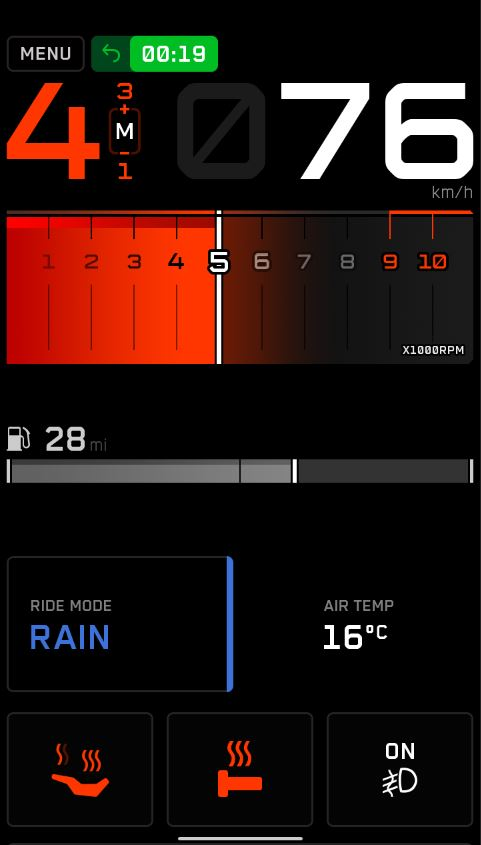
\includegraphics[width=0.3\textwidth]{Figures/Portrait_MainScreenPSD.JPG}
    \caption{KTM \gls{db} frame that includes some of the required assets like speed, air temperature and fuel range.}
    \label{KTM_DB_Unlabelled}
\end{figure}

\subsubsection{\gls{dc} Method Selection}
In \gls{od} projects, the methods of collecting the data are directly impacting not only the quality and quantity of the \gls{ds} but also the overall project cost and development time. Different \gls{dc} methods can be selected to ensure project efficiency:

\begin{itemize}
    \item \textbf{Crowed Sourcing}: This method is effective when a large and diverse image or video \gls{ds} within a limited time frame needs to be collected. Contributors are reached through online platforms to collect labeled and unlabeled data. This method benefits from scalability, cost and time effectiveness and diversity of the \gls{ds}. However, it suffers from problems like lack of quality consistency and requires effective quality control mechanisms to ensure the quality \cite{AIMultiple_Computer_Vision_Training_Data}.
    \item \textbf{Private Collection}: Private \gls{dc} refers to gathering data internally within a controlled environment. This method is used when highly customized \gls{ds} is required to ensure hat the data is tailored to specific project needs. The advantages of this method include higher data quality, better control over labeling accuracy and compliance with privacy or security requirements. However, it is relatively expensive and time-consuming \cite{AIMultiple_Computer_Vision_Training_Data}.
    \item \textbf{Off-The-Shelf \gls{ds}s}: Off-the-shelf \gls{ds} are publicly available, pre-collected \gls{ds} that researchers and developers can use directly for training and evaluation. The main advantages of using off-the-shelf \gls{ds} are that they are cost effective, easy to access and often come with high quality annotations. However, challenge is the limited customization as they may not match the project requirements \cite{AIMultiple_Computer_Vision_Training_Data}.
    \item \textbf{Generative \gls{ai}}: Generative \gls{ai} refers to \gls{ai} models that create synthetic data, including images, text and videos. this data can be used to augment \gls{ds} or generate entirely new training samples. Advantages include the ability to generate diverse and controlled data, reduce the need for real world \gls{dc} and enhance model generalization. However, challenges include the risk of synthetic data not perfectly representing real world conditions and environmental factors and inability to generate highly specific data for a specific product \cite{AIMultiple_Computer_Vision_Training_Data}.
\end{itemize}

Since the data required for this project is highly specific to the KTM \gls{db} and must comply with the privacy and security requirements. Therefore, the private collection method was chosen as the most suitable approach.

\subsubsection{High Quality Data Preparation}
To ensure that the data collected for an \gls{od} project is of high quality, several key factors must be considered. One of the most important factors is data diversity, as it directly impacts the model’s ability to generalize to real-world variations. To enhance model robustness, the \gls{ds} should include diverse objects, frames, positions, and lighting conditions during the \gls{dc} process. Additionally, accurate annotation with labels and bounding boxes is essential for enabling the model to correctly classify and localize objects within an image. A balanced \gls{ds} is also crucial to prevent model bias toward specific classes; therefore, an equal number of images per object class should be maintained. Furthermore, high-resolution and distortion-free images positively impact the model’s performance by ensuring clearer object features and reducing noise in training data.



\subsection{Data Annotation And Labeling}
........
\subsection{Dataset Preprocessing}
.........
\subsection{Augmentation Techniques}
........

\section{Object Detection And Classification Algorithm}
.........
\subsection{Overview Of Object Detection Pipeline}
.........
\subsection{Selection Of the Pretrained Model}
.........
\subsection{Data Preprocessing And Augmentation}
.........
\subsection{Model Fine-Tuning And Training Process}
..................
\subsection{Post-Processing And Object Classification}
.........
\subsection{Model Evaluation Metrics}
.........
\section{Test Setup}
.........
\subsection{Camera System}
.........
\subsection{Light Control And Mounting}
.........
\subsection{Hardware In The Loop System}
.........
\section{Integration Techniques}
.........
\subsection{Algorithm Integration With Camera System}
.........
\subsection{Synchronization With Hardware In The Loop System}
.........
\subsection{Data Flow And Processing Pipeline}
.........
